\documentclass[../elettronica]{subfiles}

\begin{document}
%Lezione 7

\section{Transistore bipolare a giunzione BJT}
\label{section:transistor_bjt}
\begin{figure}[h]
    \centering
    \begin{circuitikz}[scale=1.5]
        \draw
        (0, 0) to[diode, v=$V_{BC}$, i<=$I_C$] (2, 0) node[above]{$C$}
        (0, 0) to[diode, v=$V_{BE}$, i=$I_E$] (-2, 0) node[above]{$E$}
        (0, 0) to[short, i<=$I_B$] (0, -1) node[right]{$B$}

        (0, 0) node[circ]{}
        ;
    \end{circuitikz}
    \caption{transistor bipolare}
    \label{circit:transistor_bjt}
\end{figure}
\subsection{Modello di Ebers e Moll}
Supponiamo che $V_{BE} > 0$ e $V_{BC} < 0$. Questo ci permetterà di dire che il diodo tra base
ed emettitore è polarizzato in regione diretta ed il diodo tra base e collettore è polarizzato
in inversa.
Questo comporta che $I_E > 0$ e $I_C \approx 0$ e, considerando la legge di Kirchoff $I_B + I_C = I_E$,
abbiamo $I_B \approx I_E$.

Quello che accade se la distanza tra i due diodi è ridotta (che indicheremo con $w$), l'interazione tra
le loro cariche porta fa cambiare loro comportamento radicalmente, portando a far valere le
relazioni $I_e \approx -I_c$ e $I_b \approx 0$.


Quando $w$ è sufficientemente piccolo, quello che accade è che nel momento in cui il diodo tra base ed emettitore è' polarizzato
in diretta, ed il diodo tra base e collettore è polarizzato in inversa, la corrente fluisce prevalentemente fra collettore
ed emettitore a fronte di una corrente di base molto più piccola rispetto alle altre due regioni.
% 9:40

\begin{wrapfigure}{r}{.4\textwidth}
    \centering
    \vspace{-2\baselineskip}
    \begin{circuitikz}[/tikz/circuitikz/bipoles/length=1cm]
        \draw
        (0, 0)
        to[short, i=$\I{BC}$] (0.7, 0)
        to[diode] (2, 0)
        to[short, i<=$\I{C}$] ++(0.5, 0) node[below]{$C$}
        (0, 0)
        to[short, i=$\I{BE}$] (-0.7, 0)
        to[diode] (-2, 0)
        to[short, i=$\I{E}$] ++(-0.5, 0) node[above]{$E$}
        (0, 0) to[short, i<=$\I{B}$] (0, -1) node[right]{$B$}

        (0, 0) node[circ]{}
        ;
        \draw[clr-main-red] (2, 0)
        to[short, i=${\I{t}}$, color=clr-main-red] (2, 1)
        to[american controlled current source, color=clr-main-red] (-2, 1)
        -- (-2, 0)
        ;

        \draw[clr-primary] (-2, 1)
        -- (-2, 1.8)
        to[american controlled current source, color=clr-primary] ++(4, 0)
        -- (2, 1)
        ;
    \end{circuitikz}
\end{wrapfigure}
\vspace{10pt}
Possiamo tenere conto di questo comportamento attraverso un generatore aggiuntivo di corrente (riportato in rosso) che aggiunga
alla corrente prevista dal modello del diodo polarizzata in inversa, correntemente trascurabile, una nuova corrente
che dipende a sua volta esponenzialmente da \vbe. Chiameremo questa corrente $I_t$: corrente dell'\textbf{effetto transistore}.

\vspace{20pt}
\begin{tcolorbox}[title={Equazioni caratteristiche transistore}, width=\textwidth]
    \begin{align*}
        &\I{BE} = \diodecurrent[\I{BES}]{\V{BE}}\\
        &\I{BC} = \diodecurrent[\I{BCS}]{\V{BC}}\\
        &\I{t} = {\color{clr-main-red} \diodecurrent[\I{S}]{\V{BE}}} - {\color{clr-primary} \diodecurrent[\I{S}]{\V{BC}}}
    \end{align*}
\end{tcolorbox}

\vspace{10pt}
\noindent È semplice calcolare l'espressione della corrente di emettitore $\I{E}$, di collettore $\I{C}$ e di base $\I{B}$,
attraverso le equazioni di Kirchoff ai tre nodi.
Bisogna considerare che abbiamo utilizzato solo una particolare condizione di polarizzazione.
Se studiassimo il caso opposto, ovviamente otterremmo risultati simmetrici: vedremo che con $\V{BE} < 0$ e $\V{BC} > 0$
avremo una componente aggiuntiva di corrente ad effetto transistore, diretta in direzione opposta, rappresentabile anch'essa
con un generatore di corrente pilotato.

%17:39
\begin{tcolorbox}[title=Equazioni caratteristiche transistore (linearm. dipendenti)]
    \begin{align*}
        &\I{B} = \diodecurrent[\I{BES}]{\V{BE}} - \diodecurrent[\I{BC}]{\V{BC}}\\
        &\I{E} = \diodecurrent[(\I{S} + \I{BE})]{\V{BE}} - \diodecurrent[\I{S}]{\V{BC}}\\
        &\I{C} = \diodecurrent[\I{S}]{\V{BE}} - \diodecurrent[(\I{S} + \I{BCS})]{\V{BC}}\\
    \end{align*}
\end{tcolorbox}

\vspace{20pt}
\begin{wrapfigure}{r}{.2\textwidth}
    \vspace{-2\baselineskip}
    \begin{center}
        \begin{circuitikz}
            \draw (0, 0) node[npn](bjt){}
            (bjt.B) node[ocirc]{} node[left]{B}
            (bjt.E) node[ocirc]{} node[below]{E}
            (bjt.C) node[ocirc]{} node[above]{C}
            ;
        \end{circuitikz}
    \end{center}
    \caption{transistor npn}
    \label{component:transistor_npn}
\end{wrapfigure}

\noindent Il transistore in figura \ref{component:transistor_npn} prevede due giunzioni ed ha il nome di \textbf{transistore npn}.
Esiste anche il suo duale, \textbf{transistore pnp} al quale faremo solo un rapido cenno più avanti ma suo
comportamento è del tutto identico a quello che stiamo discutendo.

Per la legge di Kirchoff abbiamo se conosciamo due tra le differenze di potenziale ai lati del transistore, la terza è
univocamente determinata. Ragionamento del tutto analogo vale per le correnti.

Per determinare completamente il regime di funzionamento del transistore, occorre determinare le 6 grandezze: 3 correnti e 3
tensioni, attraverso 6 equazioni, due delle quali sono quelle di Kirchoff appena indicate.
Per trovare le altre quattro equazioni, utilizziamo lo stesso metodo che abbiamo applicato per determinare le
equazioni del diodo: mettiamo un morsetto a terra e, fornendo un potenziale su uno dei due morsetti rimanenti, misuriamo
il potenziale sull'ultimo morsetto.

Ovviamente è possibile connettere il transistor in 3 modi differenti: emettitore, base e collettore comune. Ma di queste
ultime due ce ne occuperemo più avanti.

\begin{figure}[h]
    \centering
    \begin{circuitikz}[scale=1.2]
        \draw (0, 0)
        to[american voltage source, v=$V_i$, i=$\I{B}$] (0, 2)
        -- (1, 2)
        -- (1, 1) node[npn, anchor=B](tr){}

        (tr.E) -- (tr.E |- 0, 0)
        (0, 0) -- (tr.E |- 0, 0)
        -- ++(1, 0) coordinate(x)

        (tr.C) -- (tr.C |- 0, 2)
        -- ++(1, 0)
        to[R, v^=$V_u$, i<=$\I{C}$] (x)
        ;
    \end{circuitikz}
    \caption{Connessione a Emettitore comune}
    \label{circuit:transistor_bjt_common_e}
\end{figure}

%37:00
\noindent Già osservando il circuito, possiamo notare che due incognite sono eliminate dalla equazione della tensione in ingresso
$\V{i} = \V{BE}$, che possiamo considerare data, e dall'equazione $\V{u} = R\cdot \I{C}$.
Ricordando che la corrente in ingresso corrisponde alla corrente di base, e che la corrente in uscita corrisponde alla
corrente di collettore, per le ultime due equazioni residue possiamo utilizzare quelle fornite dalle caratteristiche del transistore
elencate precedentemente.

\vspace{10pt}
\begin{tcolorbox}
    \begin{align*}
        &\I{B}(\V{BE}, \V{CE}) = \diodecurrent[\I{BES}]{\V{BE}} - \diodecurrent[\I{BC}]{\V{BC}}\\
        &\I{C}(\V{BE}, \V{CE}) = \diodecurrent[\I{S}]{\V{BE}} - \diodecurrent[(\I{S} + \I{BCS})]{\V{BC}}\\
    \end{align*}
\end{tcolorbox}
\vspace{10pt}
Siccome queste relazioni di correnti sono due funzioni di due variabili ($\V{BE}$ e $\V{CE}$), è necessario
un grafico in tre dimensioni per poterle rappresentare graficamente, e ciò non sarebbe pratico.

Per questo motivo riconduciamo queste espressioni ad una rappresentazione più semplice, riconducendoci ad una famiglia di curve parametriche
ponendo $\V{CE}$ come variabile indipendente e tracciando le funzioni al variare di $\V{CE}$ (Figura \ref{graph:transistor_bjt_3d}).

\newpage
\begin{figure}[h]
\begin{minipage}{.47\textwidth}
    \centering
    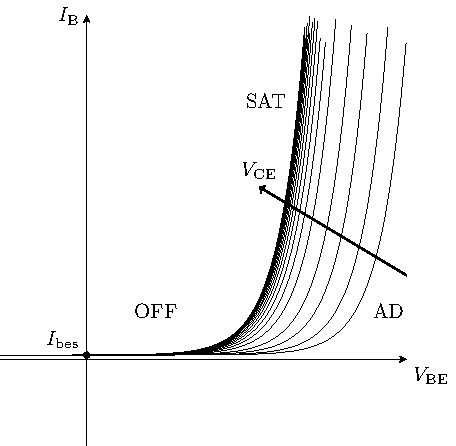
\includegraphics[width=\textwidth]{graph_bjt_ib_varying_vce}
    \caption{$\I{B}(\V{BE})$ al variare di $\V{CE}$}
    \label{graph:transistor_bjt_3d}
\end{minipage}
\begin{minipage}{.47\textwidth}
    \centering
    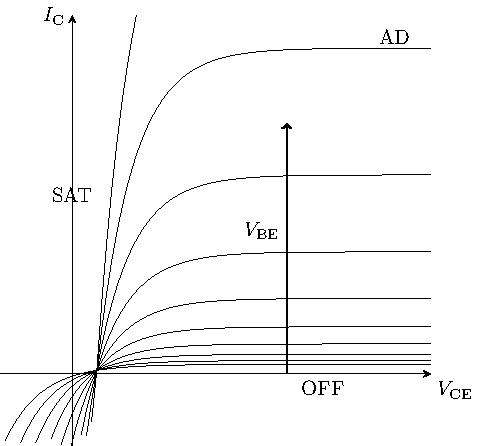
\includegraphics[width=\textwidth]{graph_bjt_ic_varying_vbc}
    \caption{$\I{C}(\V{CE})$ al variare di $\V{BE}$}
    \label{graph:transistor_bjt_3d_2}
\end{minipage}
\end{figure}

\vspace{20pt}
\noindent Il transistor è composto da 2 diodi, ognuno polarizzabile in regione diretta o regione inversa. Possiamo riconoscere quindi
quattro regioni di funzionamento del transistore, dipendenti da $\V{BE}$ e $\V{BC}$.
\begin{itemize}
    \item BE on, BC off: Regione normale di funzionamento o regione di polarizzazione attiva diretta
    \item BE off, BC on: Regione di polarizzazione attiva inversa.
    \item BE off, BC off: Regione di interdizione, per brevità diremo che il transistore è spento
    \item BE on, BC on: Regione di saturazione.
\end{itemize}

\subsubsection{Regione Attiva Diretta}
Prendendo in considerazione la regione di funzionamento attiva diretta, considerando che $e^{\V{BE} / \V{T}} > e^{\V{BC}/{\V{T}}}$
siccome il primo termine è maggiore di 1 per $\V{BE} > 0$ ed il secondo minore di 1 per $\V{BC} < 0$, possiamo semplificare le relative
equazioni caratteristiche del transistore in
\begin{align*}
    &\I{C} = \diodecurrent[\I{s}]{\V{BE}}\\
    &\I{B} = \diodecurrent[\I{BEs}]{\V{BE}}\\
    &\I{E} = \diodecurrent[(\I{s} + \I{BEs})]{\V{BE}}
\end{align*}
Osserviamo che in questa regione, tutte le correnti assumono la forma di esponenziale traslata in funzione della sola tensione $\V{BE}$.
In questo caso particolare, il circuito in figura \ref{circuit:transistor_bjt_common_e}, la corrente in uscita $\I{c}$ non è una funzione della tensione
di uscita $\V{u} = \V{CE}$, quindi si comporta come un circuito generatore di corrente costante/controllata in funzione di $\V{i}$.

Inoltre, siccome tutte le correnti dipendono dallo stesso esponenziale, allora sono proporzionali tra loro
\[
    \frac{\I{C}}{\I{B}} = \frac{\I{s}}{\I{BEs}} = \beta_F
\]
Per analogo ragionamento $\I{E} = (\beta_F+1) \I{B}$, e $\I{C} = \frac{\beta_F}{\beta_F + 1}\I{E} = \alpha_F \I{E}$.
Con $\alpha_F$ viene definita l'\textit{efficienza di emettitore}: maggiore è la costante più la corrente di collettore assomiglia alla corrente di emettitore.
Quindi siccome $\alpha_F = \frac{\beta_F}{\beta_F + 1}$, maggiore è $\beta_F$, più $\alpha_F$ è vicina ad 1, e migliore è il transistore.

\subsubsection{Regione attiva inversa}
Per ragionamento analogo alla regione precedente, $\V{BE} < 0$ e $\V{BC} > 0$ ci porta a trascurare i termini in funzione di $\V{BE}$
\begin{align*}
    &\I{C} = -\diodecurrent[(\I{S} + \I{BCs})]{\V{BC}}\\
    &\I{B} = \diodecurrent[\I{BCs}]{\V{BC}}\\
    &\I{E} = -\diodecurrent[\I{s}]{\V{BC}}\\
\end{align*}
Indicando con $\beta_R = {\I{s}}/{\I{BCs}}$, abbiamo che
\begin{align*}
    &\I{E} = - \beta_R \I{B}\\
    &\I{C} = -(\beta_R + 1) \I{B}\\
    &\I{E} = \frac{\beta_R}{1 + \beta_R}\I{C} = \alpha_R \I{C}
\end{align*}
Il crescere di $\beta_R$ aumenta le prestazioni del transistore: $\alpha_R \approx 1$.
\\[1em]
Nota: \textit{F e B a pedice, indicano Forward e Reverse}

\subsubsection{Regione di interdizione}
$\V{BE} < 0$ e $\V{BC} < 0$ ci portano ad osservare che ciascuna delle espressioni esponenziali è trascurabile, quindi:
\begin{align*}
    &\I{C} = \I{BCs}\\
    &\I{B} = - \I{BEs} - \I{BCs}\\
    &\I{E} = \I{BEs}
\end{align*}
"Il modello non ha bisogno dell'aggiunta di un generatore controllato per essere descritto".

\subsubsection{Regione di saturazione}
$\V{BE} > 0$ e $\V{BC} > 0$ indica che nessun esponenziale è trascurabile. Tutte le correnti dipendono da entrambe le tensioni di funzionamento $\V{BE}$ e $\V{BC}$.

\newpage
\subsection{Amplificatore invertente di tensione per piccoli segnali}
Utilizzando le approssimazioni appena ricavate nel circuito in figura \ref{circuit:transistor_bjt_common_e}

\begin{tcolorbox}[title=Regione attiva diretta, width=\textwidth]
    \begin{align*}
        &\vu = \vbe - \vbc > 0\\
        &\vu = -R\I{C} = -R \diodecurrent[\I{s}]{\vbe} < 0
    \end{align*}
\end{tcolorbox}

\noindent
Quindi il circuito non può funzionare in regione normale.
Modifichiamo quindi il circuito aggiungendo un generatore di tensione $\V{cc}$ tale che $\vu = \V{cc} - R\I{c} > 0$.
Mantenendo compatibilità con la prima ipotesi.

\begin{figure}[h]
    \centering
    \begin{circuitikz}[scale=1.2]
        \draw (0, 0)
        to[american voltage source, v=$V_i$, i=$\I{B}$] (0, 3)
        -- (1, 3)
        -- (1, 1.5) node[npn, anchor=B, scale=2](tr){}

        (tr.E) -- (tr.E |- 0, 0)
        node[ground]{}
        (0, 0) -- (tr.E |- 0, 0)
        -- ++(1, 0) coordinate(x)

        (tr.C) -- (tr.C |- 0, 3)
        -- ++(1, 0)
        node[circ] {} node[above] {$\vu$}
        to[R, i<=$\I{C}$] ++(0, -2)

        (x) to[american voltage source, v_=$\V{cc}$] ++(0, 1)

        ;
    \end{circuitikz}
\end{figure}
\noindent
Siccome ci siamo assicurati che il circuito funzioni in regione attiva diretta, verifichiamo ora se è possibile che tale
circuito funzioni in regione attiva inversa:

\begin{tcolorbox}[title=Regione attiva inversa]
    \begin{align*}
        &\vu = \vbe - \vbc < 0\\
        &\vu = \V{cc} - R\I{C} > 0
    \end{align*}
\end{tcolorbox}

\noindent
Abbiamo dimostrato quindi che questo circuito, corretto appositamente per farlo lavorare in regione attiva diretta,
non può lavorare in regione attiva inversa. Per funzionare in quest'ultima regione il generatore di tensione \V{cc} dovrebbe
avere una tensione negativa, per questo motivo per analizzare di questo circuito, consideriamo solo
tre regioni di funzionamento.

\noindent
\begin{minipage}{.49\textwidth}
    \begin{tcolorbox}[title=Regione di interdizione]
        \vspace{-1.5em}
        \begin{align*}
        &\I{C} = \I{BEs} \approx 0\\
        &\vu = \V{cc}\\
        &\vbe = \vi < 0\\
        &\vbc = \vi - \vu < 0
        \end{align*}
    \end{tcolorbox}
\end{minipage}
\begin{minipage}{.49\textwidth}
    \begin{tcolorbox}[title=Attiva diretta]
        \begin{align*}
        &\vbe = \vi > 0\\
        &\vu = \V{cc} - R \diodecurrent[\I{s}]{\vi}\\
        \end{align*}
    \end{tcolorbox}
\end{minipage}

\noindent
In regione di saturazione abbiamo che
\begin{align*}
    \I{C} = \frac{\V{cc} - \vce}{R}
\end{align*}
Ricordandoci che in figura \ref{graph:ramo_di_carico} abbiamo già calcolato una relazione che lega \I{C} e \vce.
Tracciamo l'equazione di $\I{C}$ appena trovata. Ciascuno dei punti di intersezione in tale figura, rappresenta
quindi il luogo dei punti soluzione di questa equazione.
Dal grafico quindi possiamo osservare che in regione di saturazione, la tensione di uscita continua a calare, ma
tende asintoticamente ad un valore appena maggiore di 0.

\begin{figure}[h]
\centering
\begin{minipage}{.48\textwidth}
    \def\vt{1}
    \def\kuno{1.250}
    \def\kdue{3}
    \begin{tikzpicture}[declare function={
            ib(\vbe,\vce) = \kuno *(e^(\vbe/\vt)-1) - \kdue *(e^((\vbe - \vce)/\vt -1));
        }]

        \begin{axis}[restrict y to domain=-1:10, ymin=-1, xmin=-1, xlabel=$\V{CE}$, ylabel=$\I{C}$]
            \foreach \i in {0.25, 0.50, ...,1.5}
            {
                \addplot {ib(\i, x)};
            }

            \addplot [solid] coordinates {(0, 3) (4, 0)};
            \draw (0, 3) node[circ]{} node[left]{$\frac{\V{cc}}{R}$}
                (4, 0) node[circ]{} node[below]{$\V{cc}$};
            \draw[->, thick] (3, 0.2)--(3, 4.5)
                node[left]{$\V{i}$};
        \end{axis}
    \end{tikzpicture}
    \label{graph:ramo_di_carico}
    \caption{Grafico con ramo di carico}
\end{minipage}
\begin{minipage}{.48\textwidth}
    \begin{tikzpicture}[declare function={
            fun(\x,\R) = (3 - \R*(exp(\x) -1)) * (\x < (3 - \R*(exp(\x) -1)))
            + (\x > (3 - \R*(exp(\x) -1)))* (exp(-\x + 1));
        }]
        \begin{axis}[ymin=-2, xmin=-2]
            \addplot[domain=-5:0]{3};
            \addplot[domain=0:5]{fun(x, 1)};
            \addplot[dashed, clr-gray]{x};
        \end{axis}
    \end{tikzpicture}
    \caption{Andamento qualitativo di \vu in funzione di \vi}
    \label{fig:bjt_graph}
\end{minipage}
\end{figure}

\noindent
In particolare, il valore a cui asintoticamente tende la tensione in uscita è dato da
\[
\I{C} = \bjtcurrentic = 0
\]
Dove entrambi i termini 1 sono trascurabili, siccome entrambi gli esponenziali sono maggiori di 1.
\[
\vce  = \V{T} \ln{\frac{1}{\alpha_R}}
\]
Quindi \vce è strettamente positivo, dato che $\alpha_R$ è compreso tra 0 ed 1, quindi il suo reciproco è maggiore di 1, e
rispettivo logaritmo è positivo.
Inoltre dato che questa espressione non dipende da \vbe, significa che tutte le caratteristiche intersecano l'asse delle ascisse
in corrispondenza di tale valore.
\\[10pt]
Considerando ora un punto $(\V{i0}, \V{u0})$ appartenente al tratto di polarizzazione attiva diretta,
la retta tangente al grafico in tale punto ha equazione $\vu - \V{u0} = m (\vi - \V{i0})$, il termine $m$, uguale alla derivata
di \vu rispetto a \vi, calcolata in $(\V{i0})$, è chiamato "guadagno di tensione" ed è indicato dal simbolo $A_V$.
\\[10pt]
Dato che la corrente $\I{c}(\V{i0}) = \I{c0} = \diodecurrent{\V{i0}}$, e siamo in regione attiva diretta (quindi il termine 1
è trascurabile rispetto all'esponenziale), possiamo dire che $\I{c0} = \I{S}e^{\V{i0}/\V{T}}$.
Quindi se calcolando il guadagno di tensione in $\V{i0}$ otteniamo:
\begin{align*}
    \vu = \V{cc} - R\diodecurrent{\vi}\\
    \frac{d\vu}{d\vi}\Bigg|_{\V{i0}} = -\frac{R \I{s}}{\V{T}}e^{\V{i0}/\V{T}}
    = -\frac{R}{\V{T}} \I{c0}
\end{align*}
Per dare una stima a questo rapporto, prendiamo ad esempio un punto intermedio, in cui $\V{u0} \approx 2.5 V$. Mentre la tensione termica
\V{T} che compare a denominatore è dell'ordine di grandezza di $25 mV$, quindi $A_V \approx -100$.
Questo valore significa che in regione attiva diretta, le piccole variazioni di un segnale in ingresso, vengono amplificate di
un fattore $A_V = 100$. Comportamento tipico di un amplificatore di tensione per piccoli segnali.
% 19:35
Ovviamente, se il segnale di ingresso raggiunge la regione di saturazione, il segnale d'uscita non sarà più sinusoidale.

Facendo riferimento ad un segnale binario, il quale può assumere solamente i valori \vh molto grande e \vl prossimo a zero, allora
il circuito si comporta come un invertitore.

\newpage
\subsection{Approssimazione Transistor BJT}
Esattamente come abbiamo fatto nel caso del diodo, approssimiamo nello stesso modo le caratteristiche del transistor bipolare.
Osservando i grafici in figura \ref{graph:transistor_bjt_3d} e \ref{graph:transistor_bjt_3d_2}, possiamo formulare un modello
lineare, valido nelle tre regioni di funzionamento, trascurando la regione inversa.
Siccome dai calcoli svolti in precedenza, sappiamo che il grafico in figura \ref{graph:transistor_bjt_3d_2} non passa per lo zero,
chiamiamo tale punto $\vcesat = 0.2 V$.
\\[1em]
Inoltre, siccome in saturazione entrambi i diodi sono in polarizzazione diretta
\[
    \vce = {\vbe}_{on} - {\vbc}_{on} = \vcesat
\]
Sapendo già che in polarizzazione diretta ${\vbe}_{on} = V_\gamma$, possiamo dire che ${\vbc}_{on} = 0.55 V = V_\gamma'$, quindi le tensioni
base-emettitore e base-collettore in polarizzazione diretta, sono diverse tra di loro.
\\[1em]
\begin{minipage}{.49\textwidth}
    \begin{tcolorbox}[title=OFF, width=\textwidth]
        \[\begin{cases*}
            \I{B} = 0 ,\quad \vbe < V_\gamma\\
            \I{C} = 0 ,\quad \vbc < V_\gamma'
        \end{cases*}\]
    \end{tcolorbox}
\end{minipage}
\begin{minipage}{.50\textwidth}
    \begin{tcolorbox}[title=AD, width=\textwidth]
        \[\begin{cases*}
            \I{B} > 0 ,\quad \V{BE} = V_\gamma\\
            \I{c} = \beta_F \I{B} > 0, \quad \vce > \vcesat
        \end{cases*}\]
    \end{tcolorbox}
\end{minipage}
\begin{tcolorbox}[title=SAT]
    \[\begin{cases*}
        \I{B}> 0, \quad \vbe = V_\gamma\\
        \I{C} < \beta_F \I{B} , \quad \vce = \vcesat
    \end{cases*}\]
\end{tcolorbox}

\noindent
In questo caso, siccome abbiamo a che fare con due giunzioni, abbiamo bisogno di definire due correnti, e per ciascuna delle regioni
abbiamo due disequazioni che descrivono la validità delle due equazioni.

\subsubsection{Studio del circuito utilizzando il modello approssimato}
\begin{minipage}{.32\textwidth}
    \begin{tcolorbox}[title=OFF]
        \[\begin{cases*}
            \vu = \V{cc}\\
            \vi < V_\gamma
        \end{cases*}\]
    \end{tcolorbox}
\end{minipage}
\begin{minipage}{.33\textwidth}
    \begin{tcolorbox}[title=AD]
        \vspace{-1em}
        \[\begin{cases*}
            \vcesat < \vu < \V{cc}\\
            \vi = V_\gamma
        \end{cases*}\]
    \end{tcolorbox}
\end{minipage}
\begin{minipage}{.33\textwidth}
    \begin{tcolorbox}[title=SAT]
        \[\begin{cases*}
            \vi = V_\gamma\\
            \vu = \vcesat
        \end{cases*}\]
    \end{tcolorbox}
\end{minipage}
\begin{wrapfigure}{r}{0pt}
    \begin{tikzpicture}[scale=.8]
        \begin{axis}[ymin=-1, xmin=-1, ymax=4]
            \addplot[domain=-5:\vgamma]{3};
            \addplot coordinates {(\vgamma, 3) (\vgamma, \vcesatval)};
            \draw (\vgamma, \vcesatval) node[circ]{};
        \end{axis}
    \end{tikzpicture}
\end{wrapfigure}

\vspace{1em}
\noindent
Questo modello rappresenta il tratto a pendenza elevata, con un tratto a pendenza infinita (tratto verticale).
Se stiamo progettando un' amplificatore analogico, il quale si basa sul determinare il guadagno del
circuito ($A_V$), non è una buona approssimazione.

Inoltre il modello rappresenta tutta la regione di saturazione con un unico punto, di coordinate $(V_\gamma, \vcesat)$
quindi è un'approssimazione non accettabile.

La spiegazione di questo fenomeno è che, siccome $\lim_{\vi \to \infty} \I{C} = \infty$ non esiste un asintoto verticale,
mentre noi stiamo approssimando tutte le possibili relazioni corrente-tensione con un unica retta verticale.

%1h:05
Se osserviamo per quali ordini di grandezza di corrente, questo modello non rappresenta accuratamente il valore della
tensione in uscita, sono dell'ordine dei giga ampere. Il circuito visto ora, non è realistico perché non ci sono limitazioni
per i valori di corrente \I{B}, aggiungiamo quindi una resistenza alla base, per limitare la corrente, e rianalizziamo il
circuito con il modello lineare.

\newpage
\subsubsection{Analisi dello stesso circuito con corrente limitata}

\begin{figure}[h]
    \centering
    \begin{circuitikz}[scale=1.2]
        \draw (0, 0)
        to[american voltage source, v=$V_i$, i=$\I{B}$] (0, 3)
        -- (1, 3)
        to[R, label=$R_b$] (1, 1.5) node[npn, anchor=B, scale=2](tr){}

        (tr.E) -- (tr.E |- 0, 0)
        node[ground]{}
        (0, 0) -- (tr.E |- 0, 0)
        -- ++(1, 0) coordinate(x)

        (tr.C) -- (tr.C |- 0, 3)
        -- ++(1, 0)
        node[circ] {} node[above] {$\vu$}
        to[R, i<=$\I{C}$, label=$R_C$] ++(0, -2)

        (x) to[american voltage source, v_=$\V{cc}$] ++(0, 1)

        ;
    \end{circuitikz}
\end{figure}

%1h:13
\noindent
\begin{minipage}{.5\textwidth}
    \begin{tcolorbox}[title=OFF]
        \vspace{1.2em}
        \[\begin{cases*}
            \vu = \V{cc}\\
            \vi < V_\gamma
        \end{cases*}\]
    \end{tcolorbox}
    \begin{tcolorbox}[title=AD]
        \vspace{-1.2em}
        \[\begin{cases*}
            \vi > V_\gamma \\
            \vu = \V{CC} - \frac{\beta_F R_C}{R_B} (\vi - V_\gamma)\\
            \vu > \vcesat
        \end{cases*}\]
    \end{tcolorbox}
    \begin{tcolorbox}[title=SAT]
        \[\begin{cases*}
            \vu = \vcesat\\
            \vi > \frac{R_b}{R_c}(\vcesat - \V{c}) + V_\gamma
        \end{cases*}\]
    \end{tcolorbox}
\end{minipage}
\begin{minipage}{.48\textwidth}
        \centering
        \begin{tikzpicture}[scale=.8]
            \begin{axis}[ymin=-1, xmin=-1, ymax=4]
                \addplot[dashed, clr-gray]{\vcesatval};

                \addplot[domain=-5:\vgamma]{3};
                \addplot[domain=\vgamma:3]{(3 - \vcesatval) / (\vgamma - 3) * x +3 -(3 - \vcesatval) / (\vgamma - 3) * \vgamma };
                \addplot[domain=3:5]{\vcesatval};

                \draw
                    (-0.5, \vcesatval) node[above]{\vcesat}
                    (-0.5, 3) node[above] {\V{cc}}
                    (3, 0) node[below]{$V^*$}
                    (1.9, 1.9) node[right]{AD}
                    (4, \vcesatval) node[above]{SAT}
                    (0.4, 3) node[below]{OFF}
                    ;
            \end{axis}
        \end{tikzpicture}
\end{minipage}

\noindent
Il modello a soglia descrive con un ottima approssimazione i casi in cui la corrente si mantiene limitata.
Il guadagno in questo modello lineare è esattamente il coefficiente angolare del tratto in regione attiva diretta: $-\beta_F R_C / R_B$.
Dato che dipende solamente dai valori delle due resistenze del circuito, è possibile aumentare o diminuire arbitrariamente il
guadagno introducendo una resistenza variabile nel circuito.
\subsubsection{Valutazione metodo di approssimazione}
% 1h:36 - trovare un metodo per comprendere se l'approssimazione del modello a soglia è accettabile
\begin{wrapfigure}{r}{0pt}
    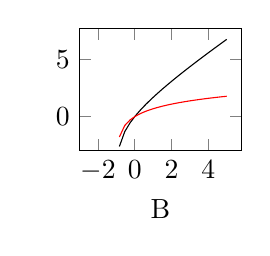
\begin{tikzpicture}
        \begin{axis}[xmin=-3, ymin=-3, ylabel=\vi, xlabel=\I{B}, width=.3\textwidth]
            \addplot[domain=-2:5]{x + ln(x + 1)};
            \addplot[domain=-2:5, color=red]{ln(x+1)};
        \end{axis}
    \end{tikzpicture}
    \caption{test}
    \label{graph:voltage_current}
\end{wrapfigure}
Mettendo insieme l'equazione di tensione e corrente della maglia in ingresso:
\begin{align*}
    &\vi - R_B \I{B} - \vbe = 0\\
    &\I{B} = \diodecurrent[\I{BEs}]{\vbe}
\end{align*}
ottengo $\vi = R_B \I{B} + \V{T} \ln(\I{B} / \I{BES} + 1)$.
\\
Si può vedere dall'espressione come la corrente di base influenza la tensione
in ingresso con un termine logaritmico ed uno lineare,
seguendo l'andamento del grafico nero in figura \ref{graph:voltage_current}.
Ad $\I{B} > 0$ la tensione in ingresso ha un andamento pressoché lineare, quindi
una variazione lineare di tensione corrisponde ad una variazione lineare di corrente.
Ciò significa che la corrente in ingresso è dissipata più facilmente sulla resistenza
che sulla giunzione base-emettitore.
Diverso è il caso precedente, rappresentato dal grafico rosso, dove per mancanza di
resistenza a piccole variazioni della tensione in ingresso corrispondono grandi variazioni
di corrente, e siccome manca la resistenza in ingresso, per raggiungere la stessa
quantità di corrente è necessario raggiungere valori di tensione molto più elevati.

\warnbox{
    Riassumendo: Quando la giunzione è in serie ad una resistenza qualunque variazione in ingresso si scarica prevalentemente
    sulla resistenza consentendo un'approssimazione di tensione costante.
    Nel caso in cui manchi la resistenza, non si può pensare di applicare un modello che consideri la tensione in ingresso costante
    se quest'ultima è variabile per definizione.
}
%1h:48m:50s - Esempio con molle

\end{document}
